% Original book p36; original base PDF p40; input PDF p51; p036_s03 六、动脑筋
% Role: question; original field: diagrams[0].tikz
% Compile with XeLaTeX from this figures/ directory.
\documentclass[12pt,tikz,border=5pt]{standalone}
\usepackage{fontspec}
\setmainfont[Path=../fonts/]{DroidSansFallback.ttf}
\setsansfont[Path=../fonts/]{DroidSansFallback.ttf}
\usepackage{amsmath,amssymb}
\usepackage{tikz}
\usetikzlibrary{calc,angles,quotes,arrows.meta,decorations.pathreplacing,decorations.pathmorphing,decorations.markings,patterns,positioning,fit,backgrounds,matrix,intersections,shapes.geometric}
\begin{document}
\color{black}
\tikzset{every picture/.append style={color=black}}
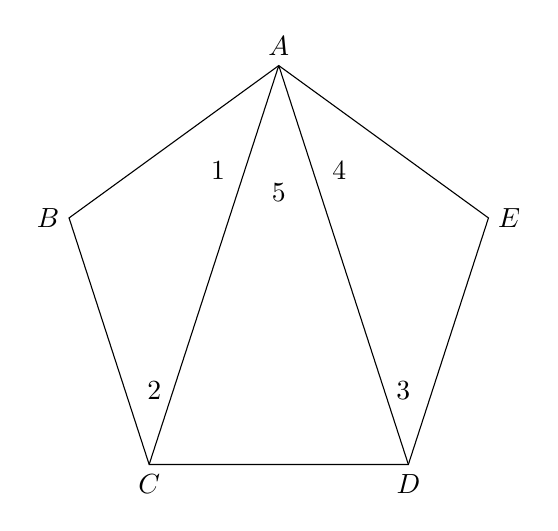
\begin{tikzpicture}[scale=1.4]\coordinate(A)at(90:2);\coordinate(B)at(162:2);\coordinate(C)at(234:2);\coordinate(D)at(306:2);\coordinate(E)at(18:2);\draw(A)--(B)--(C)--(D)--(E)--cycle;\draw(A)--(C) (A)--(D);\node[above]at(A){$A$};\node[left]at(B){$B$};\node[below]at(C){$C$};\node[below]at(D){$D$};\node[right]at(E){$E$};\node at(-.55,1.05){1};\node at(-1.13,-.95){2};\node at(1.13,-.95){3};\node at(.55,1.05){4};\node at(0,.85){5};\end{tikzpicture}

\end{document}
